El preprocesamiento de texto es un paso fundamental que implica la transformación y limpieza de datos de texto para que sean más adecuados y efectivos para su análisis por algoritmos de aprendizaje automático. Aquí hay algunas técnicas comunes utilizadas en el preprocesamiento de texto en NLP:

\begin{itemize}

	\item Segmentación de oraciones: Dividir texto en oraciones individuales implica identificar los límites entre oraciones basándose en reglas gramaticales, puntuación (como puntos, signos de interrogación, etc.) y contextos lingüísticos. Pero si el texto que se quiere dividir no contiene puntos, comas o cualquier otro carácter que indique un límite se debe encontrar alguna otra manera de dividirlo ``Como regla simple, podemos segmentar oraciones dividiendo el texto en oraciones cuando aparecen puntos y signos de interrogación. Sin embargo, puede haber abreviaturas, formas de direcciones (Dr., Sr., etc.), o elipses (...) que pueden romper la simple regla. Afortunadamente, la mayoría de las bibliotecas de PNL vienen con algún tipo de división de oraciones y palabras implementada. Una biblioteca de uso común es Natural Language Tool Kit (NLTK)''. \cite[p.50]{vajjala2020practical}.

	\item Word tokenization: implica dividir un texto en unidades más pequeñas llamadas ``tokens''. Estos tokens suelen representar palabras individuales, aunque en algunos casos pueden ser partes más pequeñas de palabras, números, signos de puntuación, etc. La tokenización se realiza típicamente antes de aplicar cualquier análisis o modelado de texto.

	\item Lematización y derivación: La derivación consiste en reducir las palabras a una forma más simple, para reducir la variabilidad y normalizar el texto. Ver parte derecha de la Figura \ref{fig:nlp2}.``La derivación se refiere al proceso de eliminar sufijos y reducir una palabra a alguna forma básica por ejemplo: ``auto'' y ``autos'' se reducen a ``auto'' Esto se logra aplicando un conjunto fijo de reglas, la derivación se usa en la clasificación de textos para reducir el espacio de funciones para entrenar modelos de aprendizaje automático.''\cite[p. 53]{vajjala2020practical}.


Lematizar es un proceso que consiste en reducir las palabras a sus formas base. Por ejemplo ``eres'' se lematiza como ``ser''. Aunque se parece a la derivación la principal diferencia radica en el proceso mucho más exhaustivo que implica no solamente eliminar sufijos o reducir la palabra.Ver Figura \ref{fig:nlp2} ``La lematización es el proceso de mapear todas las diferentes formas de una palabra a su palabra base, o lema. La lematización requiere más conocimiento lingüístico, y modelar y desarrollar lematizadores eficientes sigue siendo un problema abierto en la investigación de PNL incluso ahora.'' \cite[p. 53]{vajjala2020practical}.

\begin{figure}[h!]
	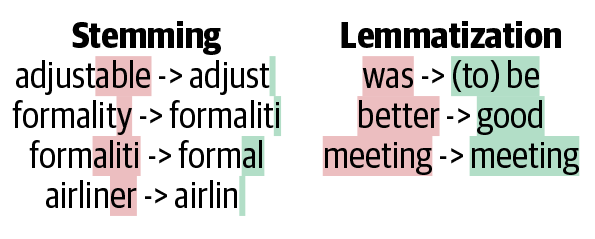
\includegraphics[width=0.65\textwidth]{capitulo3/figuras/nlp2.png}
	\caption[Diferencias entre la derivación y lematizacion]{Diferencias entre la derivación y lematizacion
		\\\textit{Fuente: Extraído de} \protect\cite[p. 54]{vajjala2020practical}}
	\label{fig:nlp2}
\end{figure}
	
	\item Eliminar caracteres no alfabéticos: Eliminar signos de puntuación, números, símbolos, direcciones web y otros caracteres no alfabéticos simplifica el texto para un análisis y procesamiento más sencillo. La eliminación de estos caracteres innecesarios reduce el ruido en el análisis, mejorando la calidad y precisión de los modelos. Para esta tarea específica, el uso de expresiones regulares en funciones es altamente recomendado, ya que el tratamiento de cada conjunto de datos es diferente, debido a que cada uno tiene sus propias particularidades.
	
	\item Minúsculas: Transformar todo el texto en minúsculas es importante para unificar el tratamiento de palabras. Esta normalización del texto asegura una representación uniforme de las palabras bajo un mismo sistema de codificación, evitando que el modelo distinga entre palabras escritas con mayúsculas o minúsculas. Además, reduce la carga computacional al disminuir la cantidad de palabras distintas que el modelo necesita procesar, lo que mejora la eficiencia del análisis.

	\item Eliminar stopwords: Eliminar palabras comunes (stopwords) que no agregan valor al análisis, como ``el'', ``la'', ``y'', etc. Estas palabras son frecuentes en el lenguaje y aparecen en casi todos los textos. Al eliminarlas, se reduce la dimensionalidad del espacio de características y hace que el enfoque se centre en palabras clave y términos más significativos para el análisis.
	
	\item Corrección de errores ortográficos: Identificar y corregir errores ortográficos puede mejorar la precisión del análisis. Su efectividad puede variar dependiendo del contexto y del propósito del análisis. En entornos donde la precisión en la escritura es esencial, como la traducción automática o el análisis de sentimientos, corregir los errores ortográficos puede ser beneficioso. En ciertos casos, especialmente en análisis de texto informal o en redes sociales, conservar los errores ortográficos puede ser importante para capturar el tono o el estilo del texto original.
	
	\item Tratamiento de emojis: Los emojis son representaciones visuales cuya presencia puede ser crucial para comprender el tono, la intención o las emociones expresadas en un texto. En algunos casos, es útil eliminar los emojis del texto si no aportan información relevante para la tarea de procesamiento o análisis. En otros casos los emojis pueden mapearse a palabras o frases que describan su significado o intención. Por ejemplo, un emoji sonriente podría ser mapeado a la palabra ``feliz'' o ``contento'', mientras que un emoji de tristeza podría mapearse a ``triste'' o ``decepcionado''. 
Si no se decide hacer ninguno de los pasos anteriores y se considera mantenerlos en su estado original es importante convertir estos caracteres especiales a una representación más simple para su tratamiento.``Para analizar dichos símbolos no textuales y caracteres especiales, utilizamos la normalización Unicode. Esto significa que el texto que vemos debe convertirse en alguna forma de representación binaria para almacenarlo en una computadora. Este proceso se conoce como codificación de texto. Ignorar los problemas de codificación puede provocar errores de procesamiento en el futuro.''\cite[p. 45]{vajjala2020practical}.

\end{itemize}

El preprocesamiento de texto es esencial para preparar los datos de texto para su análisis, ayudando a eliminar ruido, reducir la dimensionalidad y mejorar la calidad de los datos, antes de aplicarlo a modelos de aprendizaje automático en tareas de NLP. También es importante mencionar que cada uno de los pasos de tratamiento de texto ya detallados no son obligatorios en su aplicación, que aplicar, en qué momento u orden depende solamente de lo que le convenga a la tarea que se quiere realizar 
	
	
	
